%*****************************************
\chapter{Introduction}\label{int:introduction}
%*****************************************
% This just prints the text and line width for me.
%textwidth: \printinunitsof{in}\prntlen{\textwidth}\\
%linewidth: \printinunitsof{in}\prntlen{\linewidth}
% For this document, text width = line width = 4.65015in

\section{Introduction}

Statistical analysis is the core of nearly all research projects and researchers have a wide variety of statistical tools that they can use, like \textit{SPSS}, \textit{SAS}, and \textit{R}. Unfortunately, these analysis tools are expensive or difficult to master so this lab manual introduces \acs{PSPP}, an open source statistical analysis program that is free of charge and easy to use. Even though \acs{PSPP} looks like an acronym it is not. Those letters are intended to imply that it is the opposite of \acs{SPSS} in the sense that it is provided free of charge but is compatible with the \acs{SPSS} language and datasets.

Before downloading and diving into \acs{PSPP} there are two important background fundamentals that must be considered: hypothesis and data.

\section{Discussion}

\subsection{Hypothesis}\label{intro:Hypothesis}

A hypothesis is an attempted explanation for some observation and is often used as a starting point for further investigation. For example, imagine that a physician notices that babies born of women who smoke seem to be lighter in weight than for women who do not smoke. That could lead to a hypothesis like ``smoking during pregnancy is linked to light birth-weights.'' As another example, imagine that a restaurant owner notices that tipping seems to be higher on weekends than through the week. That might lead to a hypothesis that ``the size of tips is higher on weekends than weekdays.'' After creating a hypothesis a researcher would gather data and then statistically analyze that data to determine \textit{if} the hypothesis is true but additional investigation may be needed to explain \textit{why} it is true.

In a research project there are usually two related competing hypotheses: the \textit{Null Hypothesis} and the \textit{Alternate Hypothesis}. 

\begin{itemize}
  \item Null Hypothesis (abbreviated $ H_{0} $). This is sometimes described as the ``skeptical'' view; that is, the explanation for some observed phenomenon is mistaken. For example, the null hypothesis for the smoking mother observation mentioned above would be ``smoking has no effect on a baby's weight'' and for the tipping observation would be ``there is no difference in tipping on the weekend.''
  \item Alternate Hypothesis (abbreviated $ H_{a} $). This is the suggested explanation for an observed phenomenon. In the case of the smoking mother mentioned above the alternative hypothesis would be that ``smoking causes a decrease in birth weight.'' This is called the ``alternate'' because it is different from the status quo which is encapsulated in the null hypothesis.
\end{itemize}

One commonly used example of the difference between the null and alternate hypothesis comes from the trial court system. When a jury deliberates about the guilt of a defendant they start from a position of ``innocent until proven guilty,'' which would be the null hypothesis. The prosecutor is asking the jury to accept the alternate hypothesis, or ``the defendant committed the crime.'' 

For the most part, researchers will never conclude that the alternate hypothesis is true. There are always confounding variables that are not considered but could be the cause of some observation. For example, in the smoking mothers example mentioned above, even if the evidence indicates that babies born to smokers are lighter in weight the researcher could not state conclusively that smoking caused that observation. Perhaps non-smoking mothers had better health care, perhaps they had better diets, perhaps they exercised more, or any of a number of other reasonable explanations not related to smoking. 

For that reason, the result of a research project is normally reported with one of two phrases similar to these: 

\begin{itemize}
  \item \textit{The null hypothesis is rejected.} If the evidence indicates that there is a significant difference between the status quo and whatever was observed then the null hypothesis would be rejected. For the ``tipping'' example above, if the researcher found a significant difference in the amount of money tipped on weekends compared to weekdays then the null hypothesis (that is, tipping is the same on weekdays and weekends) would be rejected.
  \item \textit{The null hypothesis cannot be rejected.} If the evidence indicates that there is no significant difference between the status quo and whatever was observed then the researcher would report that the null hypothesis could not be rejected. For example, if there was no significant difference in the birth weights of babies born to smokers and non-smokers then the researcher failed to reject the null hypothesis.
\end{itemize}

Often a research hypothesis is based on a prediction rather than an observation and that hypothesis can be tested to see if there is any significant difference between it and the null hypothesis. Imagine a hypothesis like ``walking one mile a day for one month decreases blood pressure.'' A researcher could easily test this by measuring the blood pressure of a group of volunteers, have them walk a mile every day for a month, and then measure their blood pressure at the end of the experiment to see if there was any significant difference.

\subsection{Data}\label{intro:TypesOfData}

\subsubsection{Types of Data}

There are four types of data, divided into two main groups, and it is important to understand the difference between them since that determines appropriate statistical tests to be used in data analysis.\footnote{\nameref{app:a}, on page \pageref{app:a}, lists all of the datasets used in this lab manual and specifies the type of data each contains.}

\begin{itemize}

  \item \textbf{Qualitative}. Qualitative data groups observations into a limited number of categories; for example, type of pet (cat, dog, bird, etc.) or place of residence (Arizona, California, etc.). Because qualitative data do not have characteristics like means or standard deviations, they are analyzed using non-parametric tests, as described in Lab \ref{hyp:nonparametric} on page \pageref{hyp:nonparametric}. Qualitative data can be further divided into two sub-types, nominal and ordinal.
  
  \begin{itemize}
    \item \textbf{Nominal}. Nominal data are categories that do not overlap and have no meaningful order, they are merely labels for attributes. Examples of nominal data include occupations (custodial, accounting, sales, etc.) and blood type (A, B, AB, O). A special subcategory of nominal data is binary, or dichotomous, where there are only two possible responses, like ``yes'' and ``no''. Nominal data are sometimes stored in a database using numbers but they cannot be treated like numeric data. For example, binary data, like ``Do you rent or own your home?'' can be stored as ``1 = rent, 2 = own'' but the numbers in this case have no numeric significance and could be replaced by words like ``Rent'' and ``Own.''
    
    \item \textbf{Ordinal}. Ordinal data, like nominal, are categorical data but, unlike nominal, the categories imply some sort of order (which is why it is called ``ordinal'' data). One example of ordinal data is the ``star'' rating system for movies. It is clear that a five-star movie is somehow better than a four-star movie but there is no way to quantify the difference between those two categories. As another example, it is common for hospital staff members to ask patients to rate their pain level on a scale of one to ten. If a patient reports a pain level of ``seven'' but after some sort of treatment later reports a pain level of ``five'' then the pain has clearly decreased but it would be impossible to somehow quantify the exact difference in those two levels. Ordinal scales are most commonly used for Likert-type survey questions where the responses are selections like ``Strongly Agree'', ``Agree'', ``Neutral'', ``Disagree'', ``Strongly Disagree''. Ordinal data are also used when numeric data are grouped. For example, if a dataset included respondents' ages then those numbers could be grouped into categories like ``$ 20-29 $'' and ``$ 30-39 $.'' Those groups would typically be stored in the dataset as a single number so maybe ``$ 2 $'' would represent the ages ``$ 20-29 $,'' which would be ordinal data.
  \end{itemize}

  \item \textbf{Quantitative}. Quantitative data are numbers, typically counts or measures, like a person's age, a tree's height, or the number of widgets sold. Quantitative data are measured with scales that have equal divisions so the difference between any two values can be calculated. Quantitative data are discrete if they are represented by integers, like the count of words in a document, or continuous if they are represented by fractional numbers, like a person's height. Because quantative data has characteristics like means and standard deviations, they are analyzed using parametric tests, as described in Lab \ref{hyp:parametric} on page \pageref{hyp:parametric}. Quantitative data can be further divided into two sub-types, interval and ratio\footnote{\acs{PSPP} lumps both Interval and Ratio data into a single type called ``Scale.''}.
  
    \begin{itemize}
      \item \textbf{Interval}. Interval data use numbers to represent quantities where the distance between any two quantities can be calculated but there is no true zero point on the scale. One example is a temperature scale where the difference between $ 80 $\textdegree and $ 90 $\textdegree is calculated to be the same as the difference between $ 60 $\textdegree and $ 70 $\textdegree. It is important to note that interval data do not include any sort of true zero point, thus zero degrees Celsius does not mean ``no temperature,'' and without a zero point it is not reasonable to make a statement like $ 20 $\textdegree is twice as hot as $ 10 $\textdegree.
    
      \item \textbf{Ratio}. Ratio data, like interval data, use numbers to describe a specific measurable distance between two quantities; however, unlike interval data, ratio data have a true zero point. A good example of the use of ratio data is the sales report for an automobile dealership. Because the data are a simple count of the number of automobiles sold it is possible to compare one month to another. Also, since the scale has a true zero point (it is possible to have zero sales) it is possible to state that one month had twice the sales of another.
    \end{itemize}
\end{itemize}
  
\subsubsection{Shape of Data}

\paragraph{About The Normal Distribution (Bell Curve)}\label{int:normal_distribution}

When the quantitative data gathered from some statistical project are plotted on a graph they often form a ``normal distribution'' (sometimes called a ``bell curve'' due to its shape). As an example, consider the Scholastic Aptitude Test (SAT) which is administered to more than $ 1.5 $ million high school students every year. Figure \ref{lab01_fig01} was created with fake data but illustrates the results expected of a typical SAT administration.

\begin{figure}[H]
  \begin{center}
    \fbox{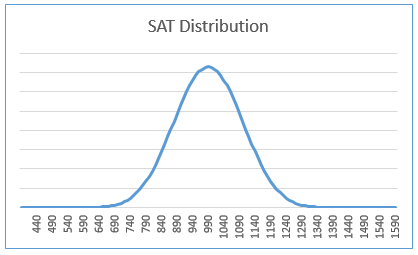
\includegraphics[width=\linewidth]{gfx/lab01_fig01}}
    \caption{Normal Distribution}
    \label{lab01_fig01}
  \end{center}
\end{figure}

SAT scores lie between $ 400 $ and $ 1600 $ as listed across the X-Axis and the number of students who earn each score is plotted. Since the most common score is $ 1000 $ that score is at the peak of the curve. Very few students scored above $ 1300 $ or below $ 650 $ and the curve is near the lower bound beyond those points. This illustrates a normal distribution where most scores are bunched near the center of the graph with only a few at either extreme.

The normal distribution is important because it permits researchers to test hypothesis about the sample. For example, perhaps a researcher hypothesized that the students in university ``A'' had a higher graduation rate than at university ``B'' because their SAT scores were higher. Because SAT scores have a normal distribution the researcher could use specific tests, like a t-test, to try to support the hypothesis. However, if the data were not normally distributed then the researcher would need to know that and select a different group of statistical tests.

\paragraph{Excess Kurtosis}
One way to mathematically describe a normal distribution is to calculate the length of the tails of a bell curve, and that is called its \textit{excess kurtosis}. For a normal distribution the excess kurtosis is $ 0.00 $, a positive excess kurtosis would indicate longer tails while a negative excess kurtosis would indicate shorter tails. Intuitively, many people believe the excess kurtosis represents the ``peaked-ness'' of the curve since longer tails would tend to lead to a more peaked graph; however, excess kurtosis is a measure of the data outliers, which would be only present in the tails of the graph; so excess kurtosis is not directly indicative of the the ``sharpness'' of the peak. It is difficult to categorically state that some level of excess kurtosis is good or bad. In some cases, data that form a graph with longer tails are desired but in other cases they would be a problem.

Following are three examples of excess kurtosis. Notice that as the excess kurtosis increases the tails become longer. 

\begin{figure}[H]
  \begin{center}
    \fbox{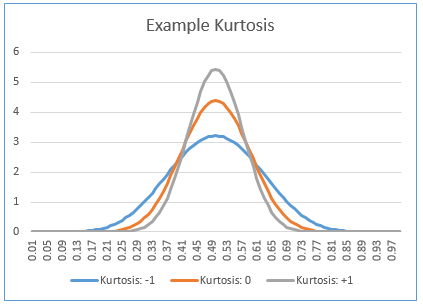
\includegraphics[width=\linewidth]{gfx/lab01_fig02}}
  \end{center}
  \caption{Kurtosis in a Normal Distribution}
  \label{lab01_fig10}  
\end{figure}

\paragraph{Skew}
The second numerical measure of a normal distribution that is frequently reported is its \textit{skew}, which is a measure of the symmetry of the curve about the mean of the data. The normal distribution in Figure \ref{lab01_fig01} has a skew of $ 0.00 $. A positive skew indicates that the tail on the right side is longer, which means that there are several data points on the far right side of the graph ``pulling'' the tail out that direction. A negative skew indicates that the tail on the left side of the graph is longer. Following are three examples of skew:

\begin{figure}[H]
  \begin{center}
    \fbox{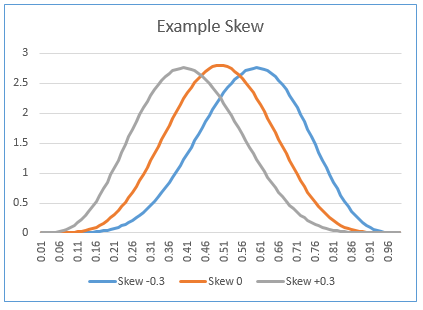
\includegraphics[]{gfx/lab01_fig03}}
  \end{center}
  \caption{Skew in a Normal Distribution}
  \label{lab01_fig13}
\end{figure}

\section{Procedure}

\subsection{Installing and Starting PSPP} 

There are versions of \acs{PSPP} available for Windows, MacOS, and Linux; so whatever operating system is being used there is a version that will work. The \acs{PSPP} downloads can be found at:

\url{https://www.gnu.org/software/pspp/get.html}. 

The download and installation process is fairly straightforward so there is no additional information about that here. Students should contact their instructor if they have trouble downloading or installing \acs{PSPP}.

\subsection{Importing Data}

For simplicity, data files that are already prepared and useable ``out of the box'' are made available with this lab manual\footnote{\acs{PSPP} can read and save \acs{SPSS} data files so students can load datasets in that format directly into \acs{PSPP} without further processing.}. Therefore, the ``Import'' feature will not be considered in this lab, but students who want to know more about importing data can find more information online. 

Students should create a single folder for all labs and store the data files in that folder. The datasets\footnote{\nameref{app:a}, on page \pageref{app:a}, details the structure and contents of all datasets used in this manual.} for all of the activities in this manual are available in a ZIP file located at:

\url{https://goo.gl/hA04Gg}

Download the ``Data Files'' for \myVersion, \myTime, and extract all of the \textbf{.SAV} files to a folder and then open them as needed.

The following datasets should be available to complete the labs in this manual:

\begin{itemize}
  \item bdims
  \item births
  \item cafe
  \item cars
  \item email
  \item gifted
  \item rivers
\end{itemize}

The description for all datasets can be found in Appendix \ref{app:a}.

\subsection{Using PSPP}

To open a dataset, click \textsc{\fbox{File $ \rightarrow $ Open}}. For example, to open the \textit{bdims} dataset:

\begin{enumerate}
  \item Start \acs{PSPP} and Click \textsc{\fbox{File $ \rightarrow $ Open}}.
  \item On the ``Select File'' screen, click \textit{bdims.sav} and then click ``Open'' at the bottom of the screen.
\end{enumerate}

When a dataset is first opened in \acs{PSPP} it is presented in a spreadsheet-like view. For example, Figure \ref{lab01_fig05} shows the top $ 10 $ rows of the cars dataset after it was first opened.

\begin{figure}[H]
  \begin{center}
    \fbox{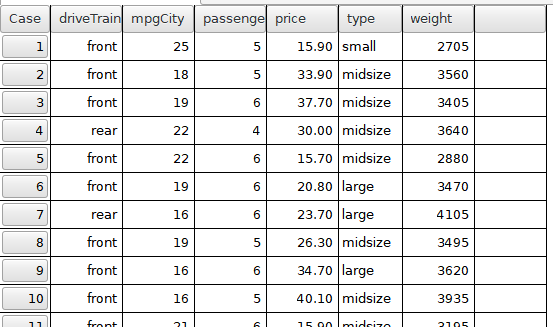
\includegraphics[width=\linewidth]{gfx/lab01_fig05}}
    \caption{The Top Of The Cars Data Table}
    \label{lab01_fig05}
  \end{center}
\end{figure}

\subsubsection{Activity 1} \label{lab01_act01}

Start \acs{PSPP} and open the \textit{cafe} dataset. Take a screen capture of the first ten rows of that data table. It should look something like Figure \ref{lab01_fig05}, which shows the top $ 10 $ rows of the \textit{cars} dataset.

\subsection{Variables}

At the bottom of the data window are two buttons used to change the window from Data View to Variable View. 

\begin{figure}[H]
  \begin{center}
    \fbox{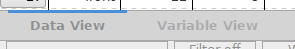
\includegraphics[]{gfx/lab01_fig06}}
    \caption{Data/Variable View Buttons}
    \label{lab01_fig06}
  \end{center}
\end{figure}

The Variable View lists all of the variables in the dataset along with the attributes for those variables. 

\begin{figure}[H]
  \begin{center}
    \fbox{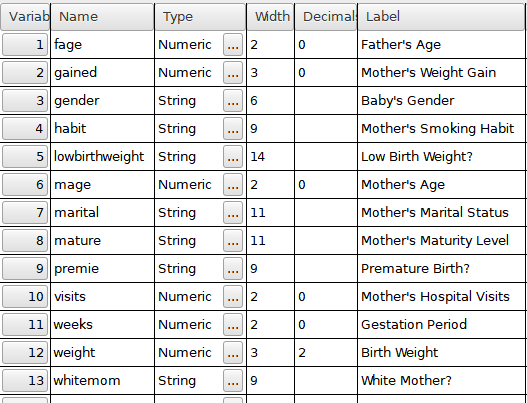
\includegraphics[width=.9\linewidth]{gfx/lab01_fig07}}
    \caption{Data/Variable View Buttons}
    \label{lab01_fig07}
  \end{center}
\end{figure}

Figure \ref{lab01_fig07} shows the first six attributes for the variables in the \textit{births} dataset, but all of the attributes are described below.

\begin{enumerate}
  \item \textbf{Variable} is simply a one-up number assigned by \acs{PSPP} when the dataset is created. 
  \item \textbf{Name} is the name of the variable. In Figure \ref{lab01_fig07}, Variable one is named ``fage.''
  \item \textbf{Type} is the type of data the variable contains. \acs{PSPP} permits the following types of data: \textit{Numeric}, \textit{Comma}, \textit{Dot}, \textit{Scientific Notation}, \textit{Date}, \textit{Dollar}, \textit{Custom Currency}, and \textit{String}\footnote{The labs in this manual use only \textit{numeric}, \textit{date}, and \textit{string} types of data.}.
  \item \textbf{Width} and \textbf{Decimal} is how much data is stored. For numeric data the Width is the size of the integer portion of the number while the Decimal attribute is the size of number's decimal portion. For \acs{PSPP} the size indicates how many places are displayed, not the size of the number. For example, the number $ 999 $ has a width of three since there are three places. For string data the width is the number of characters the variable can contain.
  \item \textbf{Label} is a label displayed in reports to make it easier to understand. For example, variable one is named ``fage'' but in a report it would be labeled as ``Father's Age'' to make it easier to understand that variable.
  \item \textbf{Value Labels} are labels for values, normally only used for nominal data. For example, it is common to store ``yes/no'' type of data where $ 0 $ is ``no'' and $ 1 $ is ``yes.'' By specifing those values as Value Labels that would be displayed in reports rather something like $ 1 $, which would be difficult to understand.
  \item \textbf{Missing Values} are how missing values should be displayed. By default \acs{PSPP} displays missing values with a dot but some sort of code could be used instead and that code is entered here.
  \item \textbf{Column} sets the width of the column displayed in the Data View.
  \item \textbf{Align} determines if a column is left, center, or right aligned.
  \item \textbf{Measure} determines how the variable is used by \acs{PSPP} and can be Scale, Ordinal, or Nominal.
  \item \textbf{Role} is the role the variable plays in the dataset. The possible roles are Input, Output, Both, None, Partition, and Split. For all of the labs in this manual the role for all variables are always ``Input.''
\end{enumerate}

Any of the above attributes can be changed but the researcher is responsible to not ``break'' the dataset by changing an attribute to an inappropriate value.

\subsubsection{Activity 2} \label{lab01_act02}

Start \acs{PSPP} and open the \textit{cafe} dataset. Switch to the \textit{Variable View} and take a screen capture of all $ 13 $ rows and the first seven columns (From \textit{Variable} to \textit{Value Labels}) of the variable view. It should look something like Figure \ref{lab01_fig07}, which shows the first six columns for the variable view of the \textit{births} dataset.

\subsection{Menus}

The top of the \acs{PSPP} screen has a menu bar with important selections. Most of the labs in this manual will focus on the \textit{Analyze} menu item. Students may also want to consider Appendix B, page \pageref{app:b}, and work through some of the \textit{Transform} menu items.

\subsection{Syntax Files}

\acs{PSPP} is, technically, a command line program with scores of commands and options that are designed to be entered in a text box. The labs in this manual, though, teach students how to use a \ac{GUI} rather than the command line. It may be easiest to think about the \ac{GUI} as a ``front end'' to the command line. Unfortunately, students who download and read the \acs{PSPP} User's Guide can quickly become confused since it discusses commands like: 

\lstinline[columns=fixed]|REGRESSION /VARIABLES={age, tip} /STATISTICS={R, ANOVA}|

with no clear relationship between a command like that and the \ac{GUI} that most students use. Technically, the \ac{GUI} is called ``PPSPIRE'' and is just an adjunct to \acs{PSPP}.

It is possible to open a command line box and manually enter commands. To access a command line box, Click \textsc{\fbox{File $ \rightarrow $ New $ \rightarrow $ Syntax}}. 

There are many commands and options available via the command line that are not available using menus in the \ac{GUI}, but those are not encountered in the labs in this manual (with only a couple of exceptions).

\section{Deliverable}

Complete the following activities in this lab:

\rowcolors{1}{gray!25}{}
\begin{center}
  \begin{tabular}{lll}
    \hline 
    \textbf{Number} & \textbf{Name} & \textbf{Page} \\ 
    \hline 
    \ref{lab01_act01} & \nameref{lab01_act01} & \pageref{lab01_act01} \\ 
    \ref{lab01_act02} & \nameref{lab01_act02} & \pageref{lab01_act02} \\ 
    \hline 
  \end{tabular} 
\end{center}

Consolidate the responses for all activities into a single document and submit that document for grading.



